%%%%%%%%%%%%%%%%%%%%%%%%%%%%%%%%%%%%%%%%%%%%%%%%%%%%%%%%%%%%%%%%%%%%%%%%%%%%%%%%
%2345678901234567890123456789012345678901234567890123456789012345678901234567890
%        1         2         3         4         5         6         7         8

%\documentclass[letterpaper, 10 pt, conference]{ieeeconf}  % Comment this line out
                                                          % if you need a4paper
\documentclass[a4paper, 10pt, conference]{ieeeconf}      % Use this line for a4
                                                          % paper

\IEEEoverridecommandlockouts                              % This command is only
                                                          % needed if you want to
                                                          % use the \thanks command
\overrideIEEEmargins
% See the \addtolength command later in the file to balance the column lengths
% on the last page of the document

% The following packages can be found on http:\\www.ctan.org
\usepackage{graphics} % for pdf, bitmapped graphics files
%\usepackage{epsfig} % for postscript graphics files
%\usepackage{mathptmx} % assumes new font selection scheme installed
\usepackage{times} % assumes new font selection scheme installed
%\usepackage{amsmath} % assumes amsmath package installed
%\usepackage{amssymb}  % assumes amsmath package installed

\usepackage{color}


\newcommand{\note}[1]{\textcolor{red}{\textbf{#1}}}

\title{\LARGE \bf
Proctor: Evaluating 3-D Recognition
}

%\author{ \parbox{3 in}{\centering Huibert Kwakernaak*
%         \thanks{*Use the $\backslash$thanks command to put information here}\\
%         Faculty of Electrical Engineering, Mathematics and Computer Science\\
%         University of Twente\\
%         7500 AE Enschede, The Netherlands\\
%         {\tt\small h.kwakernaak@autsubmit.com}}
%         \hspace*{ 0.5 in}
%         \parbox{3 in}{ \centering Pradeep Misra**
%         \thanks{**The footnote marks may be inserted manually}\\
%        Department of Electrical Engineering \\
%         Wright State University\\
%         Dayton, OH 45435, USA\\
%         {\tt\small pmisra@cs.wright.edu}}
%}

\author{Some people% <-this % stops a space
\thanks{This work was not supported by any organization}% <-this % stops a space
\thanks{H. Kwakernaak is with Faculty of Electrical Engineering, Mathematics and Computer Science,
        University of Twente, 7500 AE Enschede, The Netherlands
        {\tt\small h.kwakernaak@autsubmit.com}}%
\thanks{P. Misra is with the Department of Electrical Engineering, Wright State University,
        Dayton, OH 45435, USA
        {\tt\small pmisra@cs.wright.edu}}%
}


\begin{document}

\maketitle
\thispagestyle{empty}
\pagestyle{empty}

\begin{abstract}

REcently proliferation of cheap 3-D sensors.
Lots of work on feature representations.
But no unified evaluation available.
We present an evaluation framework for point cloud-based recognition.
Flexible as to dataset and feature.
Modular design.
Provides several metrics.
Open source.
We hope that this becomes a standard evaluation for future featurizations for 3-D recognition tasks.

\end{abstract}

%!TEX root=./report.tex
\section{INTRODUCTION}
Research in robotics and computer vision has long considered the use of 3-D point clouds as a rich source of information about the world.
Throughout the history of research, the recognition methods and features considered have shared ideas---from early work on retrieving 3-D shape models to integrating 2-D and 3-D percepts to human pose estimation.
But the sheer diversity of applications has made it hard to see the common patterns, and nearly impossible to meaningfully compare between different choices made in the processing pipeline.

\begin{figure}[thpb]
   \centering
   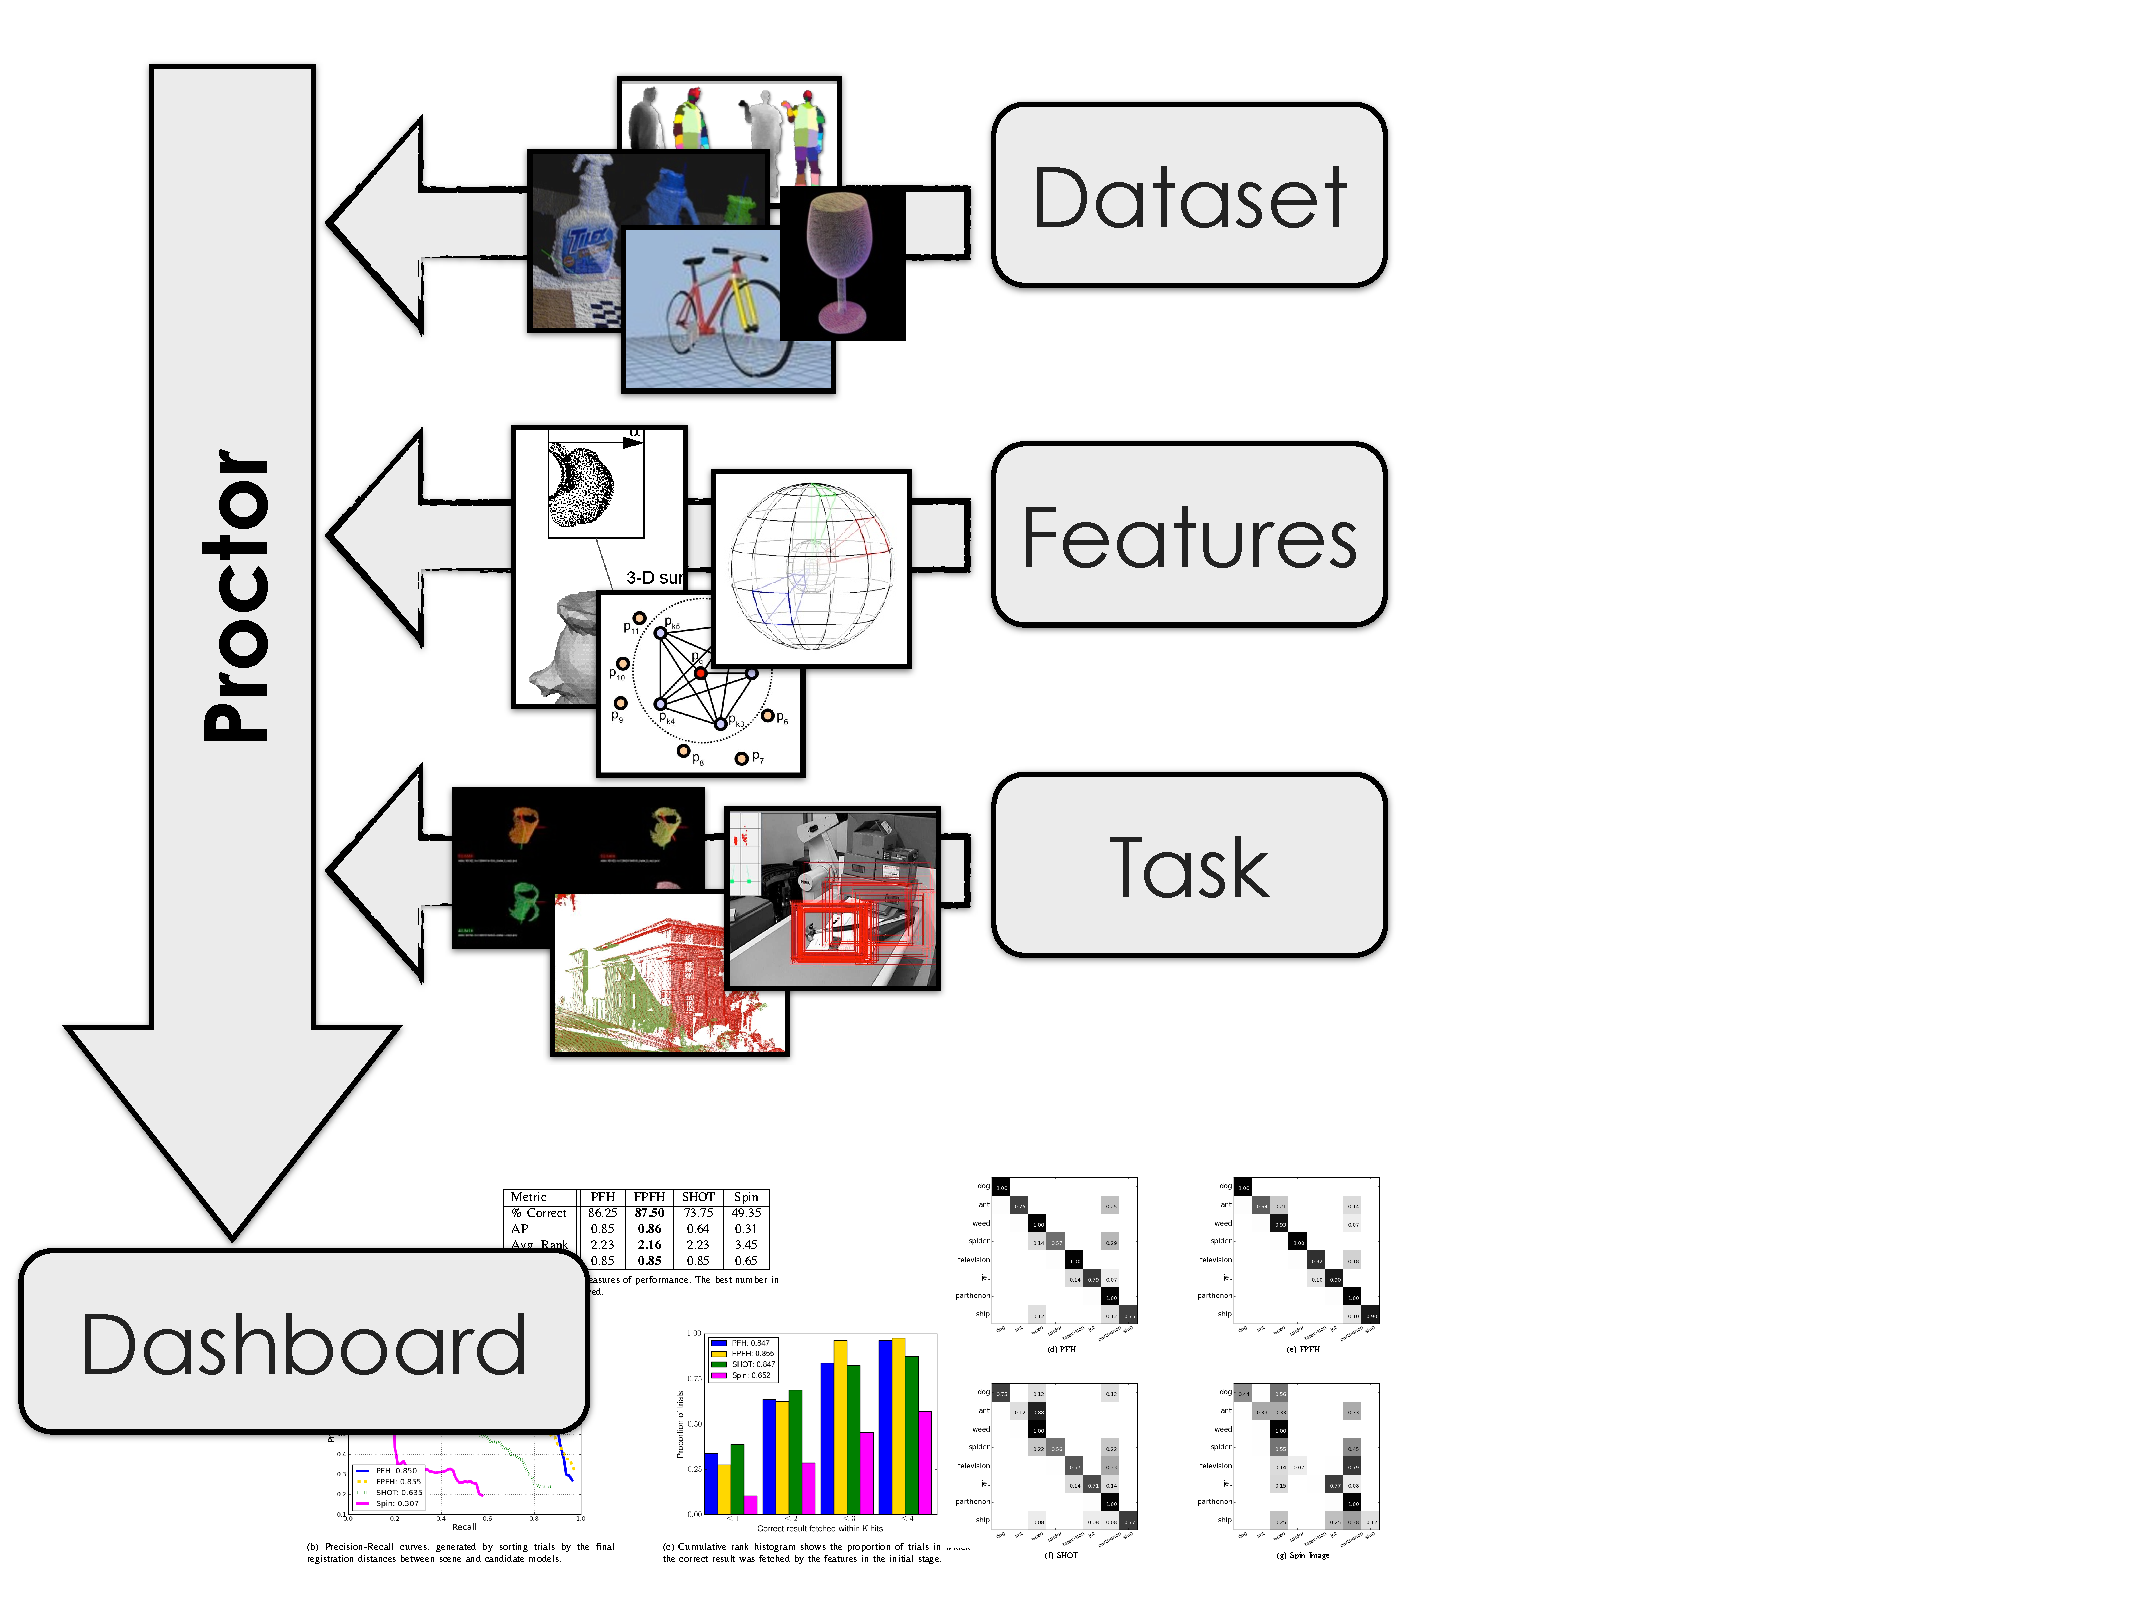
\includegraphics[width=0.45\textwidth]{../figures/figure1.pdf}
   \caption{Our system modularizes the standard 3-D recognition pipeline such that individual components may be comparatively evaluated.}
   \label{fig:figure1}
\end{figure}

We hope to foster easier sharing of ideas and methods through a common evaluation framework for 3-D perception tasks.
In this paper, we present an open-source framework for comparing different 3-D features in the model matching evaluation regime.
We explain the motivations behind our system and describe its modular architecture, with the aim of encouraging a community of users and contributors.
In robotics, the Willow Garage PR2 has facilitated rapid progress in personal robotics research due to standardization and abstraction of the hardware interface.
In computer vision, standard datasets and evaluation tasks such as the PASCAL Visual Object Challenge \cite{pascal-voc-2010} have focused research by giving groups a clear metric, and resulted in rapid improvement in object classification and detection.

Our system, Proctor, aims for the same kind of impact in 3-D features, and classification and pose estimation methods research.

\section{PROBLEM SETTING}

There is a wide range of 3-D perception problems.
While in the long run the goal of our framework is to capture this wide range more comprehensively, for now we are focused on a path through choices as given below.

Given a database and a view, our task may be to:
\begin{itemize}
\item identify the object in the view (recognition),
\item identify the object and its pose in the view (pose estimation),
\item localize an object in the view and identify it (detection).
\end{itemize}

The view provided can be clean or cluttered.
It can be solely 3-D data, or it can include an image from a camera.
The sensor that provides the 3-D data can be LIDAR, or structured light, or a stereo camera.
It can have highly regular or random noise statistics.

Our database can consist of full polygonal models, full point cloud models, or sparse views.
In the latter cases, the models may contains noise which may or may not be of the same form as our test sensor.

A common approach to all of these tasks, under many of the view and dataset conditions, is to extract local features from the 3-D data, which can then be matched to models in a database.
Matching features ``vote'' for a particular model, and subsequent algorithms can evaluate the alignment of the hypothesis model to the sensor data.

Although for launching the Proctor framework we choose to focus on
this paradigm, it is but one of many approaches to 3-D shape retrieval~\cite{Tangelder2004},
and the intent of this line of open-source work is to provide a
framework to which the community can easily contribute any 3-D shape
retrieval algorithms of interest.

We discuss a list of 3-D descriptors and various different datasets in the following subsections.

\subsection{Features}
For 3-D object detection, a feature tries to capture something about the shape of a model or a part of a model.
We considered several different features for our detector, and we summarize them here.
Some we end up evaluating with our benchmark.

The most classic feature in the 3-D perception community is the Spin Image \cite{SpinImages}.
Roughly, the name explains the feature: it's a 2-D array of values (image) that are generated by ``spinning'' the 3-D data around the normal of a point on its surface.
The motivation, as with most features, is robustness to noise and even occlusion in the task of model matching.

%(* Curvature histograms, Geometric moments)?
%Radu: not needed - all of these descriptors described here are in fact some generalization of curvature histograms


An idea related to the spin image is the 3-D shape context descriptor \cite{Frome2004}, an analog of a popular 2-D feature.
The method is to center a radially-binned sphere around a point on the surface of the 3-D data, and construct a histogram of points that fall within the bins.
The bins are weighted by distance to the center, and the bins are spaced logarithmically along the radial dimension to increase robustness to noise and clutter.

Signature of Histograms of OrienTations (SHOT)~\cite{shot} also bins points into voxels arranged around a point, but instead of contributing only mass, it keeps track of the points' orientations as well.
Thus each voxel bin is not just a number, but a histogram of its own.

Point Feature Histograms \cite{pfh1} attempt to describe a region by representing the relationships between surface normals of a k-neighborhood of the center point of the region.
The resulting feature is invariant to 6-D pose of the surface and robust to noise on the surface.
Speed is a concern for the calculation of this feature, and the Fast PFH~\cite{fpfh1} mitigates it by a recursive lookup of a simplified feature in a smaller neighborhood.

To achieve viewpoint variance, the related idea of the Viewpoint Feature Histogram \cite{Rusu2010} calculates some of the PFH-type normal angle relations with respect to the viewpoint, which is desirable for rapid object recognition.


%* An interesting simple but robust feature was used for pose recognition in the Microsoft Kinect \cite{Shotton2011}. 

One existing benchmark for features is the recent SHREC Benchmark \cite{Boyer2011} is an evaluation of 3-D feature detection and description stages of shape retrieval algorithms.
The benchmark measures how the detection and description algorithms degrade under synthetic transformations of the 3D data, including sub-sampling, isometry, holes, shot and random noise, view, and affine.
The benchmark is inspired by similar evaluation of computer vision features(\cite{Mikolajczyk2004,Mikolajczyk2005}, and the features evaluated are largely 3-D analogs of 2-D detectors and descriptors such as the Harris corner and Difference-of-Gaussians \cite{Harris1988,Lowe2004} detectors and SIFT, HOG, and MSER descriptors \cite{Lowe2004,Dalal2005,Matas2004}.


There is also research into combining 2-D and 3-D features for recognition.
Straightfoward combinations are evaluated in a household robotics task in \cite{Gould2008}.
Their method relies on high-level features derived from the 3D observation such as ``height above ground'' and simple statistics about the surface normals.
%\cite{Sun2010} shows how to benefit from 3D training data in a voting based method.
%Fritz et al. \cite{Fritz2010} extends branch\&bound to 3D and adds size and support surface constraints derived from the 3D observation.

%Most prominently, a set of methods have been proposed for fusing 2D and 3D information for the task of pedestrian detection.
%The popular HOG detector \cite{Dalal2005} to disparity-based features is extended by \cite{hattori}.
%5A late integration approach is proposed by \cite{rohrbach09dagm} for combining detectors on the appearance as well as depth image for pedestrian detection.
%Instead of directly learning on the depth map, \cite{walk10eccv} uses a depth statistic that learns to enforce height constraints of pedestrians.
%Finally, \cite{leibe10ijrr} explores pedestrian detection by using stereo and temporal information in a hough voting framework also using scene constraints.

\subsection{Datasets}
Any evaluation of a recognition algorithm depends on an appropriate dataset.
A variety of datasets are available for 3-D recognition.
They have different size, content (3D only or with 2D views), labels (pose, instance, category, or some combination of these), and source (controlled capture or ``in the wild'').
Here we summarize the most appropriate datasets for our generalized evaluation framework.

\subsubsection{3D Data Only}
{\bf Princeton Shape Benchmark \cite{Shilane2004}}:
A standard evaluation for 3-D shape retrieval, classification, and clustering applications.
The models are provided in polygonal format, and are divided into standard training and test datasets.
As for many other papers in the field, this dataset provides the evaluation basis of our implementation.

{\bf Willow Garage Grasping Database \cite{wgdb}}:
A collection of small household objects appropriate for a robot to hold.
These models are also in polygonal format.

\subsubsection{2D/3D Data}
%{\bf Rgbd-dataset of \cite{Lai2011}}:
%This dataset features 300 objects in 51 categories.
%The category count refers to nodes in a hierarchy, with, for example, ``coffee mug'' having ``mug'' as parent.
%Each category is represented by 4-6 instances, which are densely photographed on a turntable.
%For object detection, only 8 short video clips are available, which lend themselves to evaluation of just 4 categories (bowl, cap, coffee mug, and soda can) and 20 instances.
%
%%{\bf UBC Visual Robot Survey \cite{Helmer2010}}:
%%The Visual Robot Survey dataset from UBC provides training data for 4 categories (mug, bottle, bowl, and shoe) and 30 cluttered scenes for testing detection approaches.
%Each scene is photographed in a controlled setting from multiple viewpoints.

%{\bf 3D table top object dataset \cite{Sun2010}}:
%The ``3D table top object dataset'' covers 3 categories (mouse, mug, stapler) and provides 200 test images with cluttered background.
%There is no significant viewpoint variation in the test set.

{\bf Solutions in Perception Challenge \cite{SIPC2011}}:
The dataset of the ``Solutions in Perception Challenge,'' which will take place in conjunction with ICRA'12.
The goal of the challenge is to identify the extent to which 3D recognition problem is ``solved.''
It thus focuses on the high-precision part of the performance curve.
The 2011 challenge consisted of 35 distinct objects such as branded boxes and household cleaner bottles that are presented in isolation for training and in 27 scenes for test.

{\bf A Category-level 3-D Object Dataset: Putting the Kinect to Work \cite{Janoch2011}}:
An indoor, crowd-sourced dataset collected with the Kinect sensor.
The dataset aims to capture the statistics of actual household object distribution, and to be challenging by today's standards due to large viewpoint and inter-class variation, and realistic clutter in the scenes.
The first set of results is provided on 9 object classes, but the growing nature of the dataset means that more results will be published in the future.

%{\bf Other datasets:} Beyond these, a couple of other datasets have been made available which do include simultaneous capture of image and depth but serve more specialized purposes like autonomous driving \cite{ford_dataset}, pedestrian detection \cite{leibe10ijrr} and driver assistance \cite{walk10eccv}.
%Their specialized nature means that they cannot be leveraged for the multi-object category localization task that is our goal.


\section{ARCHITECTURE AND IMPLEMENTATION}
* describe the Proctor code

* synthetic approach, voting, kdTree stuff, PCL

\section{EVALUATION}

* provides the first results tables
* table per dataset
* features vs. metrics

* plots of the same data that's in the tables?

* confusion matrix figures

* table of timing results

\begin{table}
\caption{An Example of a Table}
\label{table_example}
\begin{center}
\begin{tabular}{|c||c|}
\hline
One & Two\\
\hline
Three & Four\\
\hline
\end{tabular}
\end{center}
\end{table}

\begin{figure}[thpb]
   \centering
   %\includegraphics[scale=1.0]{figurefile}
   \caption{Inductance of oscillation winding on amorphous
    magnetic core versus DC bias magnetic field}
   \label{figurelabel}
\end{figure}

\section{COMMUNITY AND FUTURE PLANS}

Open source stuff.

\section{ACKNOWLEDGMENTS}

The authors gratefully acknowledge the contribution of National Research Organization and reviewers' comments.

{\small
\bibliographystyle{ieee}
\bibliography{sergeyk-icra12,misc}
}

\end{document}
